\documentclass{beamer}
%Information to be included in the title page:
\title{Intro to RTL 2 GDSII}
\author{Nikola Petrovic}
\institute{University of Belgrade, School of Electrical Engineering}
\date{2022}

\begin{document}

\frame{\titlepage}

% 1st slide
\begin{frame}
\frametitle{Course Prerequisite}

Before taking this course, you must have experience with
\begin{itemize}
 \item<1-> Have an understanding of device physics and the IC fabrication process
 \item<1-> Have knowledge of Verilog or any other hardware description language
\end{itemize}

\end{frame}

% 2nd slide
\begin{frame}
\frametitle{Course Objective}

In this course, you 
\begin{itemize}
 \item Implement the RTL of a design from its specification
 \item Use the Xcelium™ simulator to simulate the design
 \item Verify Code Coverage using the Integrated Metrics Center
 \item Synthesize the design from RTL to Gates using the Genus™ Synthesis Solution
 \item Insert test structures to be able to test the design using the     \item Genus Synthesis Solution and verify the test coverage using the Encounter® test
 \item Compare the design against the RTL using the Conformal® Equivalence Checker
 \item Run the digital implementation flow with the Innovus™ Implementation System: 
 	\begin{itemize}
	\item Create a floorplan
	\item Implement power structures and clock trees
	\item Place-and-route the design
	\item Verify the design
	\end{itemize}
\item IRun signoff checks to make sure that the design chip can be fabricated
\end{itemize}

\end{frame}

% 3rd slide
\begin{frame}
\frametitle{Course Agenda}

\begin{itemize}
\item Design Specification and RTL Coding
\item Design Simulation Using the Xcelium Simulator
	\begin{itemize}
	\item Simulating a Simple Counter Design
	\end{itemize}
\item Code Coverage Using the Integrated Metrics Center
	\begin{itemize}
	\item Code Coverage Flow for a Simple Counter Design
	\end{itemize}
\item The Synthesis Stage
	\begin{itemize}
	\item Running the Basic Synthesis Flow
	\item Running the Synthesis Flow with DFT
	\end{itemize}
\item The Test Stage
	\begin{itemize}
	\item Running the Basic ATPG Flow in Modus Test
	\end{itemize}

\end{itemize}
\end{frame}

% 4th slide
\begin{frame}
\frametitle{Course Agenda Continued}

\begin{itemize}
\item The Equivalency Checking Stage
\begin{itemize}
	\item Running the Equivalence Checking Flow in Conformal
	\item Creating a .v Format File from .lib Format
\end{itemize}
\item The Implementation Stage
\begin{itemize}
	\item Running the Basic Implementation Flow
\end{itemize}
\item Gate-Level Simulation  
\begin{itemize}  
	\item Running Gate-Level Simulations on a Simple Counter Design
\end{itemize}
\item Timing Analysis and Debug
\begin{itemize}
	\item Using Global Timing Debug Interface to Debug Timing Results
\end{itemize}
\end{itemize}
\end{frame}

% 5th slide
\begin{frame}
\frametitle{Overview}


\begin{figure}
\centering
    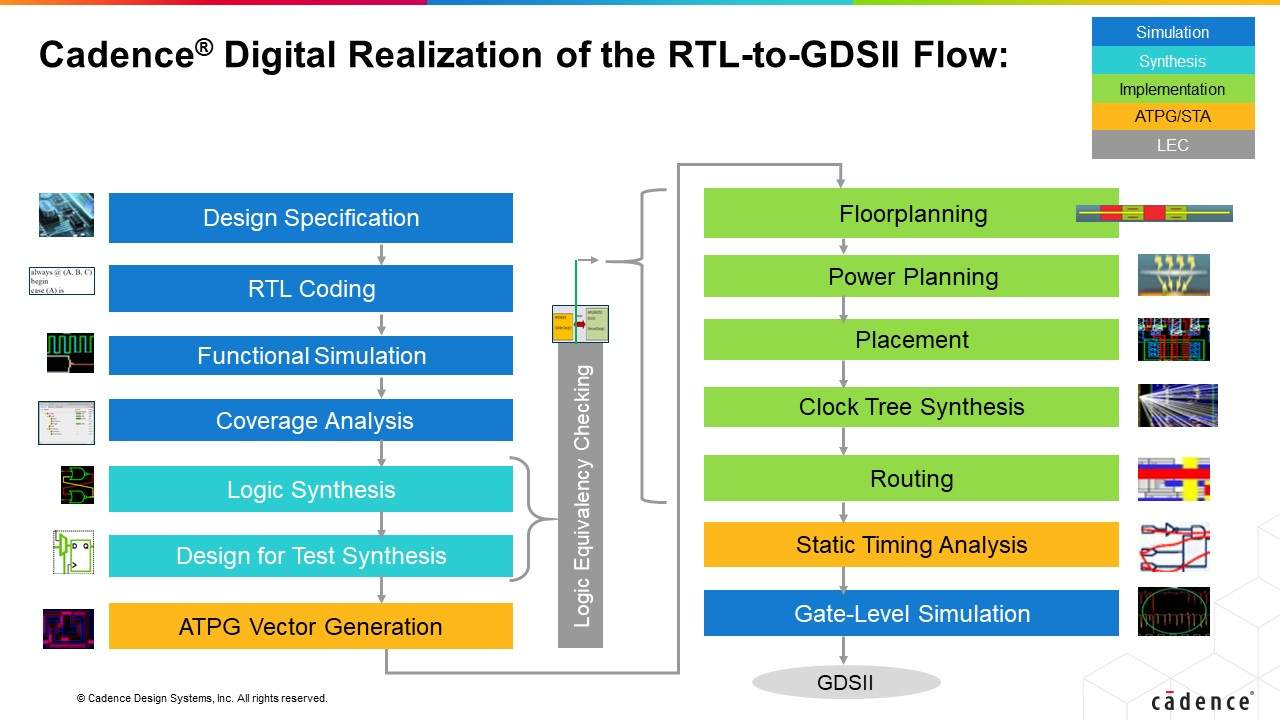
\includegraphics[width=0.95\textwidth]{overview.jpg}
    \caption{Overview of the Cadence RTL2GDSII flow.}
    \label{fig:overview}
\end{figure}

\end{frame}


\end{document}
